\documentclass{article}
\usepackage{graphicx}
\usepackage{amsmath} % For math formatting
\usepackage{amssymb}

\begin{document}

\title{Fall-2023 5304 LecN6 Notes}
\author{Wan}
\date{\today}
\maketitle

\noindent
\textbf{Topics: PD; SPD; LDLT; Cholesky Factorization.}

\section{Positive Definite Matrices}

\subsection*{Definition of PD}
A real, square matrix is said to be PD if:\\
$\left\langle Au,u\right\rangle > 0$ for all $u \neq 0$ and $u \in R^n$

\subsection*{Properties}
\textbf{1, A is nonsingular.}\\
This can be proof by contradiction.\\

\noindent
\textbf{2, The eigenvalues of A are real and positive.}\\
This can be proved by the definition of eigenvalues.\\

\pagebreak
\section{Symmetric positive definite matrices, SPD}
\subsection*{Definition of SPD}
A square matrix is SPD
if it is \textbf{symmetric} and all its eigenvalues $\lambda$ are \textbf{positive},
that is $\lambda > 0$.\\

\subsection*{Properties}
\textbf{1, Diagonal entries of SPD is positive.}\\
\\
Proof starting from the definition: Known that A is SPD, then
for all nonzero vector $u$, we have $\left\langle Au,u\right\rangle > 0$.
\noindent
Then, utilize identity matrix to extract an element of A. (MV Product, dot product view). Good enough.\\

\noindent
\textbf{2, Each $A_k$ is SPD}\\
will fill this part later.\\

\noindent
\textbf{3, a conclusion}\\
will fill this part later.\\


\noindent
\textbf{4, If A is SPD, then for any nxk matrix X of rank k, the matrix $X^TAX$ is SPD.}\\
Memory:\\
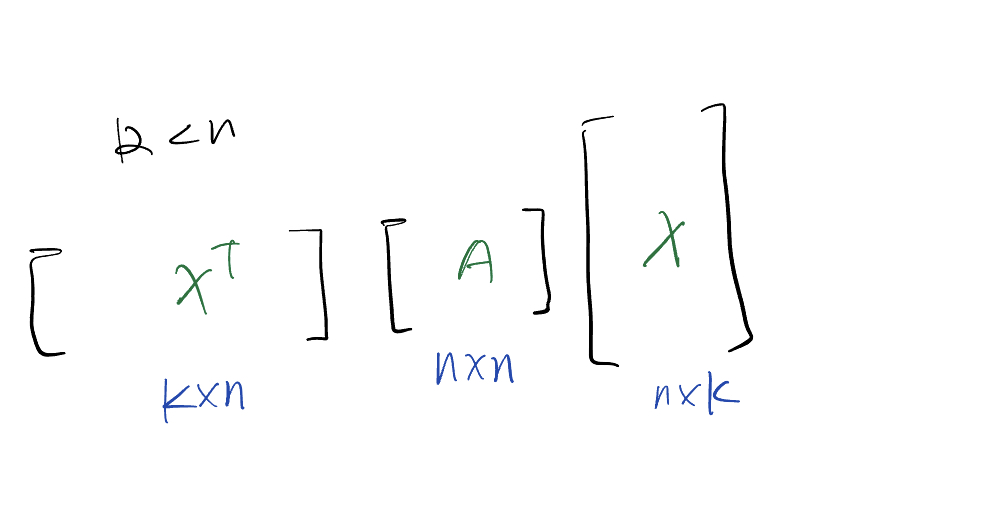
\includegraphics[width=1\linewidth]{lec6-1.jpg}
Proof (will use the notation of the inner product and def of SPD):\\




\subsection*{Application: Covariance Matrices in Statistics}

\pagebreak
\section{Pred: SPD, Semi-Definite, Neg definite, and Indefinite Matrices}


\pagebreak
\section{The $LDL^T$ Factorization from LU}

For the LU Factorization, all we need is all $A_k$ matrices for k=1 to n-1 have to
be nonsingular. As A is SPD, implying that all $A_k$ matrices from k=1 to n are nonsingular.
Thus LU fac exists and is unique.\\

\noindent
Inverse of a Diagonal Matrix is easy to compute:\\
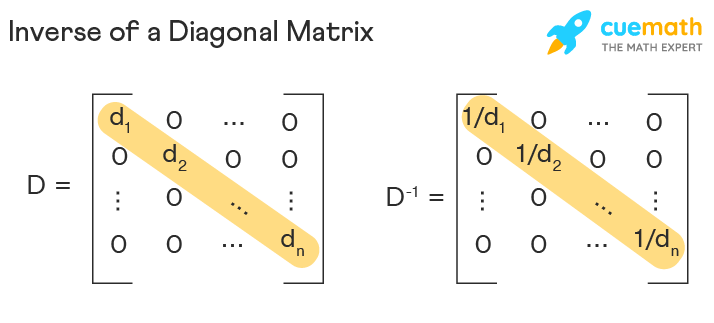
\includegraphics[width=1\linewidth]{lec6-2.png}

\noindent
Nice results because of symmetry

L is M

\noindent
Proof that $A = LU = LDL^T$\\

\noindent
Thus, a SPD matrix A could be written in this form: $A = LDL^T$
where L is a lower triangular matrix with 1s on the diagonal, and D is a diagonal matrix (of U).\\



\pagebreak
\section{The Cholesky Factorization GGT from LDLT}
Diagonal of D shoud be positive so that we can take a square root to D to reach the Cholesky.\\
\\
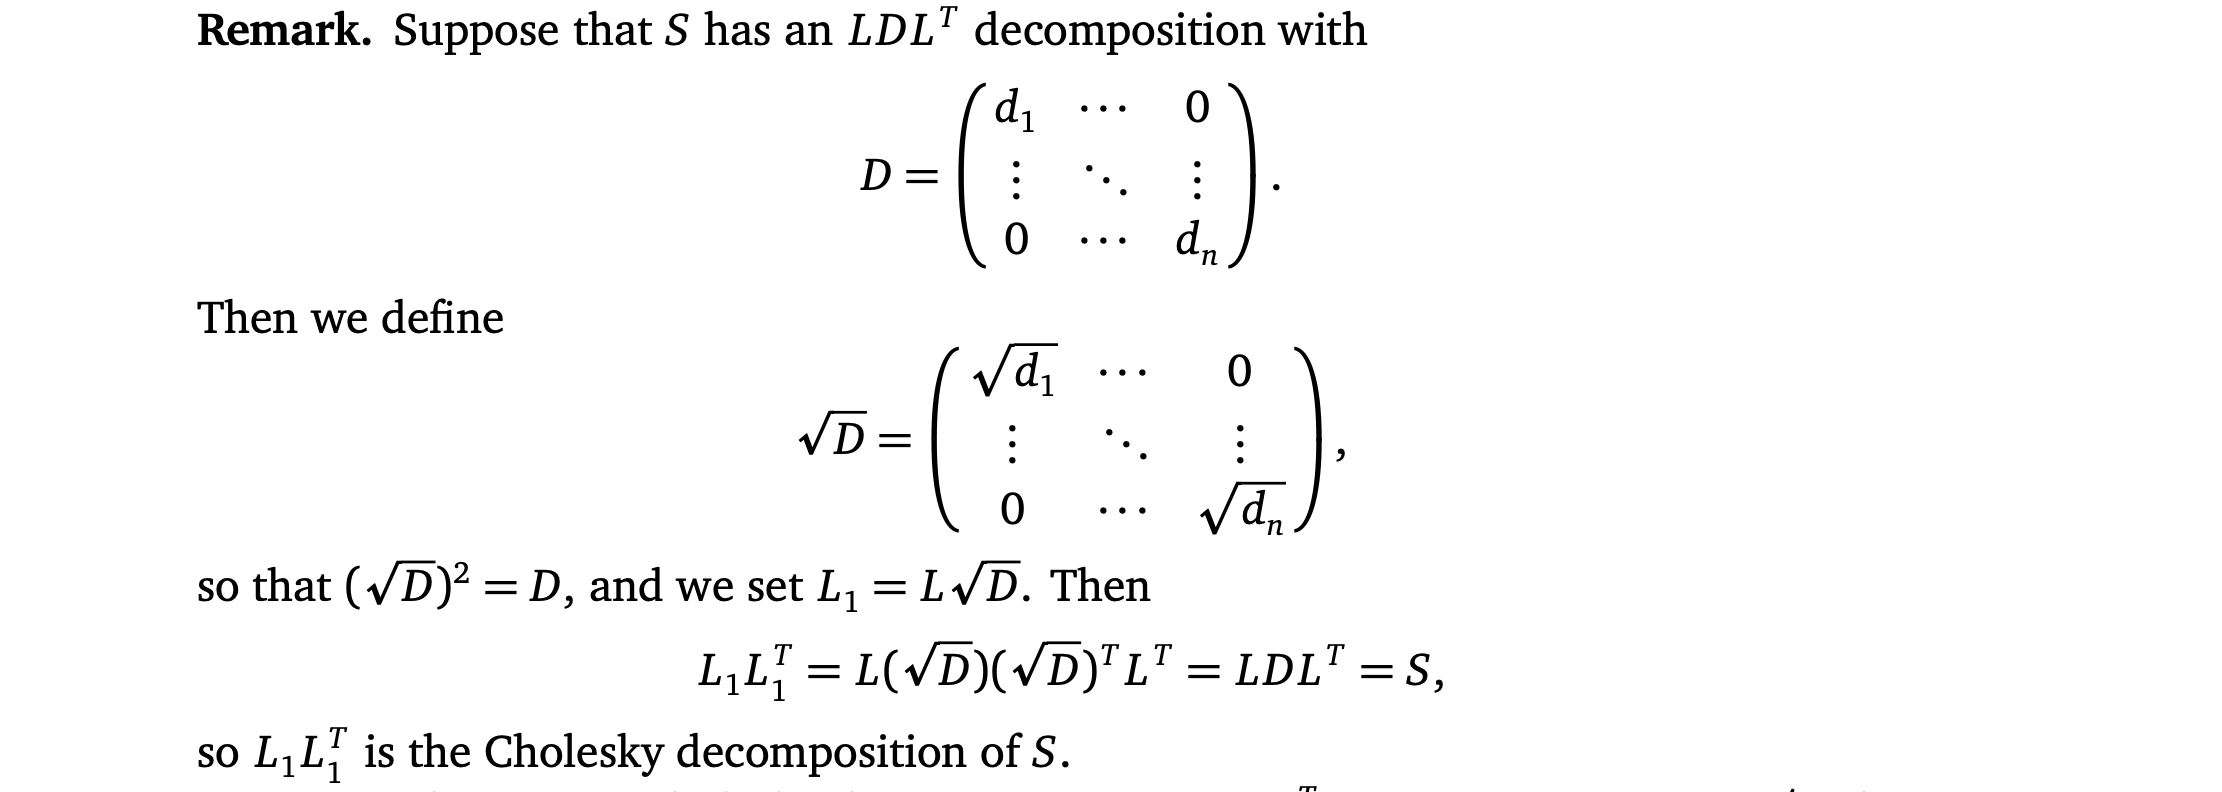
\includegraphics[width=1.5\linewidth]{lec6-3.png}\\
\\
\medskip
Proof: Diagonal of D shoud is positive


What can we say about G?
G is lower triangular

\noindent
The Cholesky: Any matrix that is SPD could be written as $A = GGT$ where G is a lower triangular matrix, and positive
entries on diagonal.\\

\subsection*{Algo of LDLT}
Idea: Just work on upper part of the matrix because of symmetry.\\

\noindent
Rank 1 update: You're updating the matrix by something like $uv^T$ where u and v are the same.\\

\end{document}